\begingroup
\setmainfont{DejaVu Sans}

\resizebox{\linewidth}{!}{%
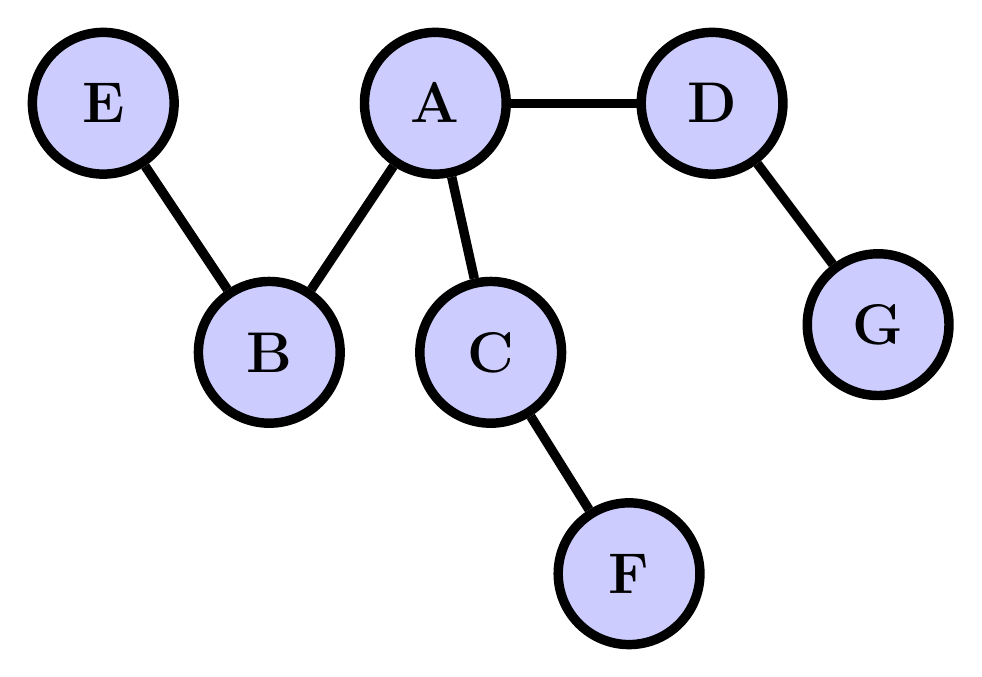
\begin{tikzpicture}
  \tikzset{
    mynode/.style={
      circle,
      draw=black,
      fill=blue!20,
      line width=1.2mm,
      minimum size=18mm,
      font=\bfseries\fontsize{20}{20}\selectfont,
      text centered
    }
  }

  \node[mynode] (A) at (0pt, 150pt) {A};
  \node[mynode] (B) at (-60pt, 60pt) {B};
  \node[mynode] (C) at (20pt, 60pt) {C};
  \node[mynode] (D) at (100pt, 150pt) {D};
  \node[mynode] (E) at (-120pt, 150pt) {E};
  \node[mynode] (F) at (70pt, -20pt) {F};
  \node[mynode] (G) at (160pt, 70pt) {G};

  \draw[line width=1.2mm] (A) -- (B);
  \draw[line width=1.2mm] (A) -- (C);
  \draw[line width=1.2mm] (A) -- (D);
  \draw[line width=1.2mm] (B) -- (E);
  \draw[line width=1.2mm] (C) -- (F);
  \draw[line width=1.2mm] (D) -- (G);
\end{tikzpicture}%
}
\endgroup

